\documentclass[a4paper]{article}

\usepackage[english]{babel}
\usepackage[utf8]{inputenc}
\usepackage{amsmath}
\usepackage{graphicx}

\title{COMP5212 Machine Learning 2018 Fall programming project \\
       \ \ \ \ \\
       Building a self-driving agent with Reinforcement Learning}

\author{Hok Chun Ng, 20272532, hcngac@connect.ust.hk \\
        Shengyuan Zhang, 20565161, szhangcg@connect.ust.hk \\
        Ge Chen, 20360858, gchenaj@connect.ust.hk}

\date{\today}

\begin{document}
\maketitle

\begin{abstract}
In this project, we build a self-driving agent that only relies on vision using deep reinforcement
learning algorithm. Due to the limitation of real-world hardware and data, we use an open
source self-driving
car simulator provided by Udacity \cite{simulator} to generate training data and testing platform.
We learn the elements of deep reinforcement learning and apply it to build our model. The results are
presented with the loss of our deep reinforcement learning model and some sample test driving traces
on the simulator.
\end{abstract}

\section{Application and practical significance}

Self-driving car has been a hot topic in recent years. Several industry giants, like Google
\cite{google} and Tesla Motor \cite{tesla}, have devoted significant efforts to the developing of
self-driving cars. 

Applications of self-driving agent can be wide. Example includes long-distance truck driving,
smart taxi and bus, or even be incorporated into large-scale autonomous traffic systems.

Letting computers to drive can release human beings from the boring and tiring job of driving as
well as reduce the frequency of traffic accidents. It also opens up new business and
city-management opportunities including smart traffic system and smart taxi services.
Applications are wide and undiscovered and the significance of perfecting self-driving agent is
huge in opening the door to these huge possibilities.

However, designing a robust self-driving system is non-trivial as the real-world traffic
conditions are diverse. Limited by hardware requirement and law, we find a solution to
self-driving in a simulated game environment in the hope that the result can be transferred to
real-world self-driving.


\section{Problem formulation}

We formulate the problem of self-driving as a continuous decision making process. The
self-driving agent receives input from sensors, evaluate each possible actions and choose
the best action.

For human drivers, the driving behavior can be formulated in a loop from an environment sensing
input to action output. Our eyes and ears are the sensors to interpret the current environment,
including the road view from wind screen (e.g. weather, traffic lights, walking people), view
from side mirror (e.g. neighboring cars, following cars), car horns, and so on. Then our brain
takes all these input signals to decide what action to take. The actions include turning the
steering wheel, lighting turn signals, accelerating, braking, and so on. Once the actions are
executed, the environment input changes, and again drivers will decide and take a new round of
actions accordingly. This loop continues until the car arrives at the destination. 

We try to mimic how human decision works with machine learning algorithms. The machine learning
problem in self-driving can be: given a set of environment input, find the best actions to
execute until arriving at destination.


\section{Udacity Self-driving car simulator }

In this project, we develop our algorithms on an open source self-driving car simulator provided
by Udacity \cite{simulator}. The simulator provides a near real-world environment of a racing 
car. The simulator can record video of every racing trace and then segment the video into image
frames. The by default sample frequency is 30 frames per second. There are two modes in the 
simulator, one is ``Training mode'' for human controlled training records and the other is ``
Autonomous mode'' for training by a machine agent. In Training mode, human player can drive the
car under simulated environment, and there is a record button to capture video and store the images.
In Autonomous mode, the control of a car can be delivered by a python program with a web socket.
The official document of Udacity provides a behavioral cloning repository \cite{behavior} to interact
with the simulation environment. 

The controls to the car include the steering angle ranging from $-25$ to $25$ and a throttle value
of $0$ and $1$. To simplify the control, we set throttle value constantly to $0$, and just apply the
steering angle control. The end of a simulation is indicated by a sudden decrease of car speed (the
highest speed in simulation is 30 miles per hour).

A sample image during training is shown in Figure \ref{fig:sample_rgb}, which is similar to a front 
view during human driving. The images are in RGB mode by default and the resolution can be set according
to a user's preference. In our scenario, we choose the $320 x 160$ as the resolution value to ease
the training burden. To further reduce training overhead, we 
also convert the RGB images to gray-scale ones. After observing the sample images, we find that
the gray-scale image data for the Red channel has better information for acting later on. 

\begin{figure}
    \centering
    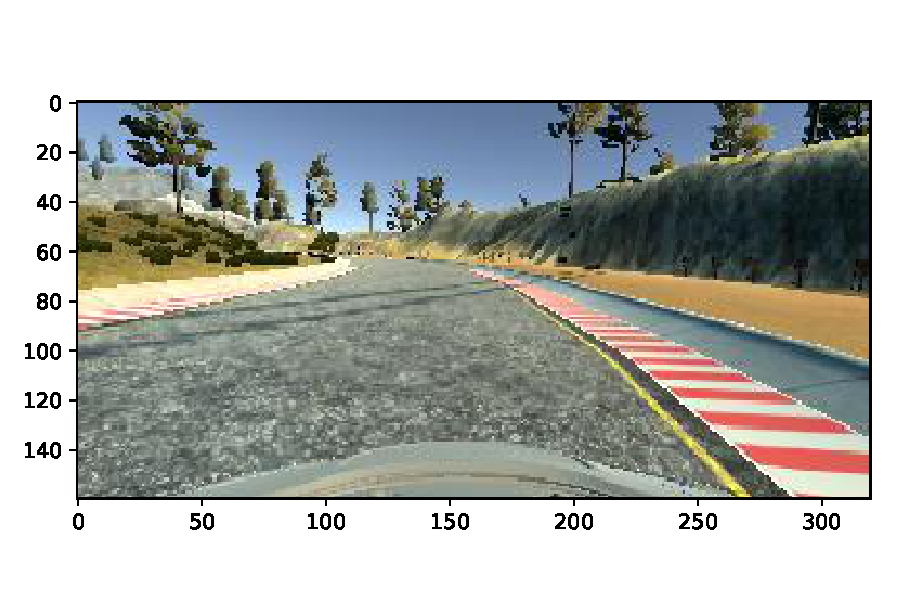
\includegraphics[width=0.8\textwidth]{./figures/sample_rgb.pdf}
    \caption{ Sample image generated by the Udacity simulator }
    \label{fig:sample_rgb}
\end{figure}


\section{Machine learning methods}

\subsection{Reinforcement learning}
The environment-action loop in the driving experience resembles the basics of reinforcement
learning, an area of machine learning concerned with taking actions in an environment in order to
maximize some notion of cumulative reward. Unlike supervised learning, reinforcement learning
does not require correct input/output pairs. Instead, reinforcement learning often requires a
reward function in terms of different actions under the environment. For driving, the final
reward can be no traffic accident and arrive at the destination safely.

\begin{figure}
    \centering
    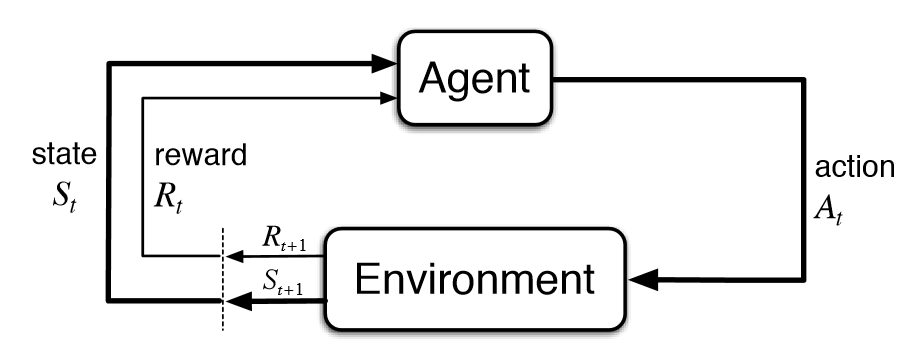
\includegraphics[width=0.8\textwidth]{./figures/rl.png}
    \caption{ Reinforcement Learning Illustration \cite{rlIntroduction}}
    \label{fig:RL}
\end{figure}



Figure \ref{fig:RL} shows the basic model of reinforcement learning \cite{rlIntroduction}. At
each time $t$, an agent receives the environment state $S_t$ and current reward $R_t$. It then
chooses an action $a_t$ from the set of available actions, which is sent to the environment. The
environment moves to a new state $S_{t+1}$ and new reward $R_{t+1}$ and feedback to the agent.
The goal of a reinforcement learning agent is to gain as much as reward as possible.

\subsection{Q learning}
Q-learning defines a reward
expectation function, $Q$, which provides the expected reward of an action $a$ taken under the
current state $s$. State is the image displayed and actions are all available actions of the
drive. This $Q$ function can be recursively defined as $Q(s,a) = R(s,a) + \alpha \max_{a^{'}}
Q(S^{'}(s,a),a^{'})$, where $R$ is the immediate reward given action $a$ taken under state $s$,
$\alpha$ is the discount rate of future reward and $S^{'}$ is the state transition.

\begin{figure}
	\centering
	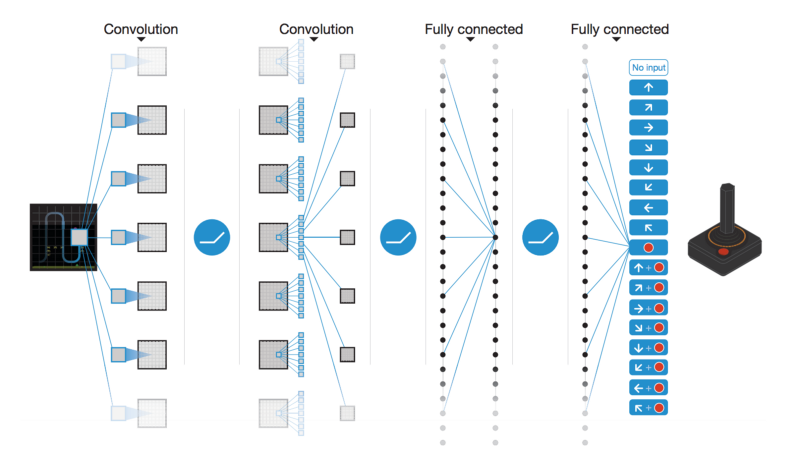
\includegraphics[width=0.8\textwidth]{./figures/deepq.png}
    \caption{ Deep Q-learning Network Illustration \cite{dqn}}
	\label{fig:deepq}
\end{figure}

\subsection{Deep Q learning}
 Deep Q learning is take a neural network to estimate the Q value for each action-reward pair. Given
numerous possibilities of imagery state $s$, we cannot compute $Q$ directly. Alternatively, we
can use a deep convolutional network to estimate $Q$.

Figure \ref{fig:deepq} illustrates a model of deep Q-learning network \cite{dqn}. First, we have
several layers of convolution and max-pooling to reduce the imagery input into smaller vector.
Then we have several fully-connected layer for the final decision making. The sample network
shown estimates a function $Q : S \rightarrow A^n$, which takes a image input and output the
expected reward for all possible actions.

\subsection{Continuous control for deep reinforcement learning}
TODO
In this project, we use the method of deep reinforcement learning for continuous control \cite{continous}.
The reason to apply this model is that our action space is the steering angle, which is a continuous 
value from $-25$ to $25$.

\section{Problem formulation}
TODO
Environment setting
Action space
Reward function

\begin{figure}
    \centering
    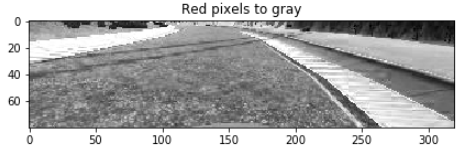
\includegraphics[width=0.8\textwidth]{./figures/sample_gray.jpg}
    \caption{ Gray-scale image data input }
    \label{fig:sample_gray}
\end{figure}


\section{Experiment and performance evaluation}
TODO
\subsection{Neural Network structure}

The sample input of our training/test model is show in Figure \ref{fig:sample_gray}.
input layers output
\subsection{Hyper-parameters}
\subsection{Loss function/ final loss value}
\subsection{Sample trained agent}
sample outputs of each layer if possible.

Our experiment involves deep Q network training and performance evaluation. 

Training is a process of random discovery. The agent is allowed to randomly choose actions in the
game until game over. States, action and reward is recorded in the process and is used to train
the deep Q network. We evaluate the performance in fixed game intervals to show the learning
progress. Training stops when the performance does not increase over certain extend.

In performance evaluation, we let the self-driving agent control the car according to the output
of the deep Q network. The agent feed the image display to the network and choose the action with
the highest output value in each step, until game over. We run the process for a number of times
to get an average performance in each evaluation. Performance is defined as the score obtained at
game over.





% \begin{figure}
% \centering
% \includegraphics[width=0.3\textwidth]{frog.jpg}
% \caption{\label{fig:frog}This frog was uploaded to writeLaTeX via the project menu.}
% \end{figure}


\begin{thebibliography}{9}
\bibitem{google}
  Google Self-Driving Car, \texttt{https://www.google.com/selfdrivingcar}

\bibitem{tesla}
  Tesla Self-Driving Hardware, \texttt{https://www.tesla.com/autopilot}

\bibitem{simulator}
  Udacity Self-driving Simulator, \texttt{https://github.com/udacity/self-driving-car-sim}

\bibitem{behavior}
  Udacity CarND Behavioral Cloning, \texttt{https://github.com/udacity/CarND-Behavioral-Cloning-P3}

\bibitem{rlIntroduction}
    Sutton, Richard S., Andrew G. Barto, and Francis Bach. \texttt{Reinforcement learning: An
    introduction.} MIT press, 1998.

\bibitem{dqn}
  Volodymyr Mnih, Koray Kavukcuoglu, et al. \texttt{Human-level control through deep
  reinforcement learning.} Nature, 2015.
  
\bibitem{continous}
   Timothy Lillicrap, Jonathan Hunt, et al. \texttt{Continuous control with deep reinforcement learning} ICLR, 2016.

\end{thebibliography}
\end{document}
